\documentclass[12pt,letterpaper]{article}
\usepackage[margin=1in]{geometry}
\usepackage{fancyhdr}
\usepackage[utf8]{inputenc}
\usepackage{palatino}
\usepackage{microtype}
\usepackage{hyperref}
\usepackage{graphicx}
\usepackage{lastpage}
\usepackage[hang,small,margin=1in]{caption}
\usepackage{titlesec}

\renewcommand{\headrulewidth}{0pt}
\fancyfoot{}
\fancyfoot[C]{\sffamily Page \thepage\ of \pageref{LastPage}}
\pagestyle{fancy}

\titleformat{\section}{\bfseries\MakeUppercase}{\arabic{\thesection}}{1em}{}
\titleformat{\subsection}{\bfseries}{\arabic{\thesection}.\arabic{\thesubsection}}{1em}{}
\titleformat{\subsubsection}{\itshape}{\arabic{\thesection}.\arabic{\thesubsection}.\arabic{\thesubsubsection}}{1em}{}

\setlength{\parindent}{0cm}
\setlength{\parskip}{1em}

\captionsetup[figure]{labelfont=it, font=it}
\captionsetup[table]{labelfont={it,sc}, font={it,sc}}

\hypersetup{colorlinks, linkcolor = black, citecolor = black, urlcolor = black}
\urlstyle{same}



\begin{document}

\fancyfoot{}
\begin{center}
    \hfill \\
    \vspace{4in}
    {\bf\Huge CS457 Project \#4 \\}
    \vspace{2in}
    {\Large Soo-Hyun Yoo \\ February 2, 2015}
\end{center}

\newpage
\fancyfoot[C]{\sffamily Page \thepage\ of \pageref{LastPage}}

\section*{Source Files}

\begin{itemize}
    \item p4.glib
    \item p4.frag
    \item p4.vert
\end{itemize}


\section*{Explanation}

\subsection*{p4.glib}


\newpage
\section*{Results}

\begin{figure}[!h]
    \centering
    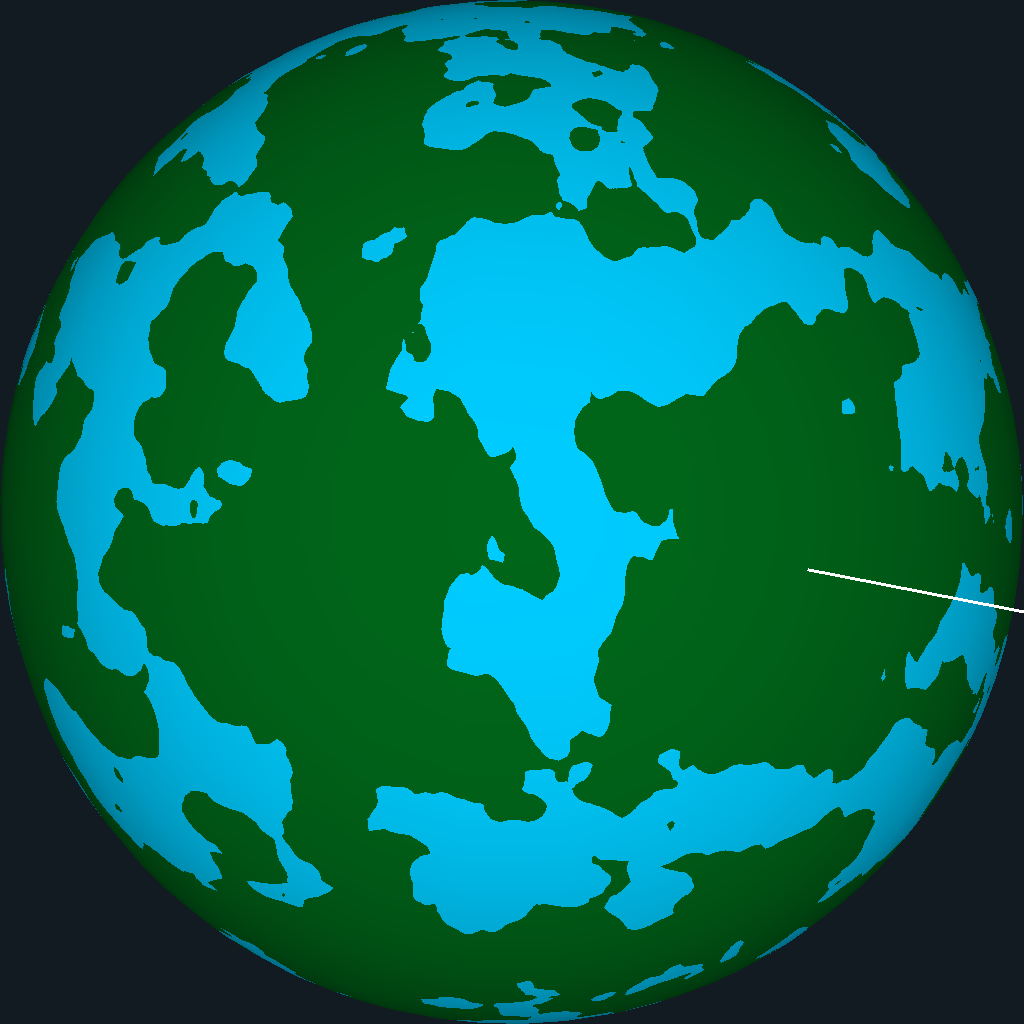
\includegraphics[width=1.0\textwidth]{img/sphere_noise.png}
    \caption{Sphere with noise.}
    \label{fig:spherenoise}
\end{figure}

\begin{figure}[!h]
    \centering
    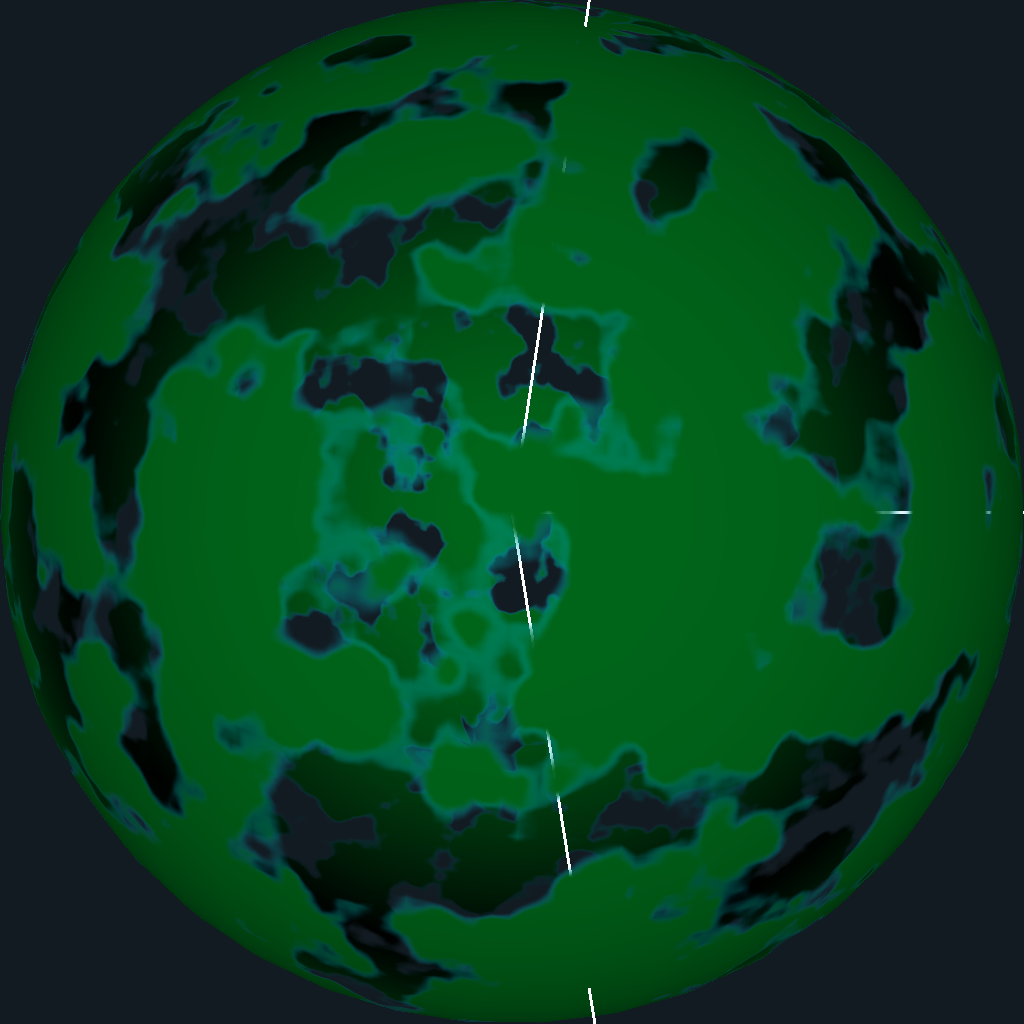
\includegraphics[width=1.0\textwidth]{img/sphere_alpha_tol.png}
    \caption{Noisy sphere with alpha and tolerance enabled.}
    \label{fig:spherealphatol}
\end{figure}

\begin{figure}[!h]
    \centering
    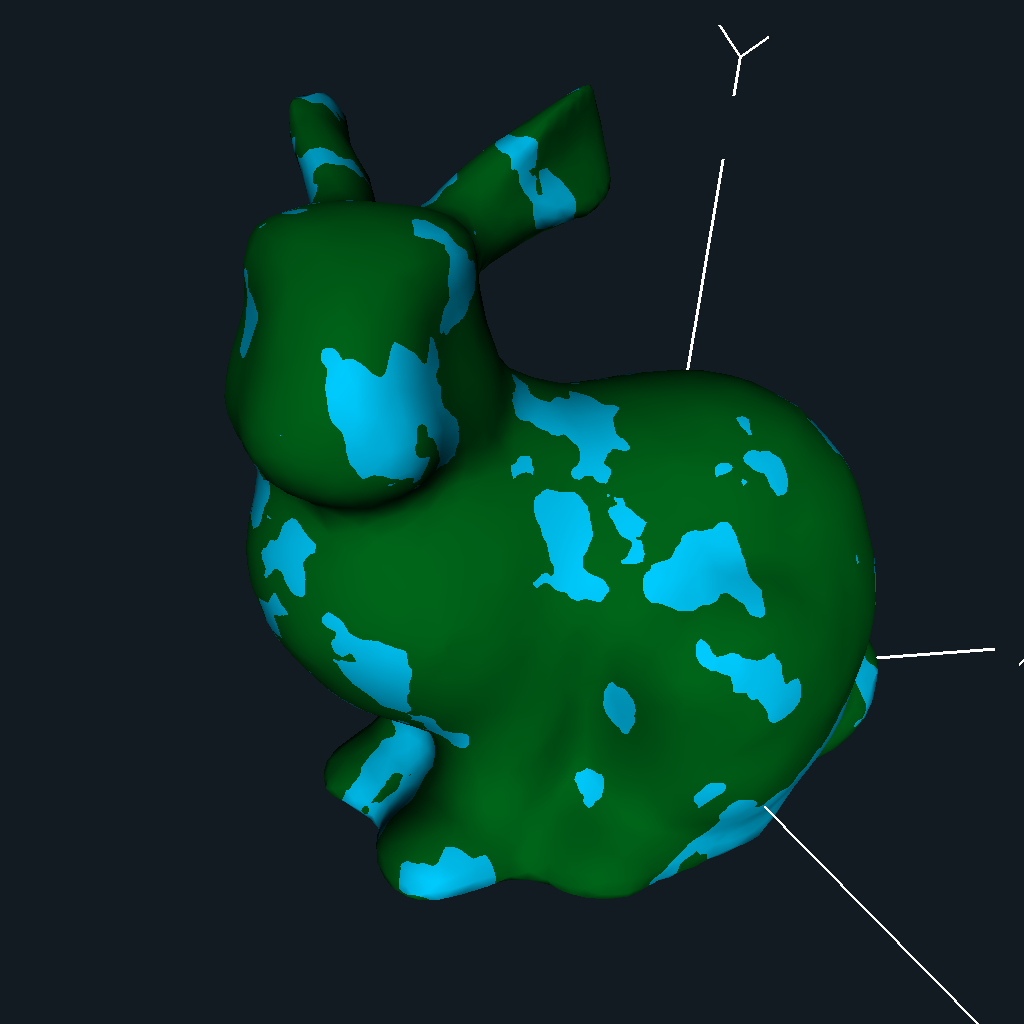
\includegraphics[width=1.0\textwidth]{img/bunny_noise.png}
    \caption{Bunny with noise.}
    \label{fig:bunnynoise}
\end{figure}

\begin{figure}[!h]
    \centering
    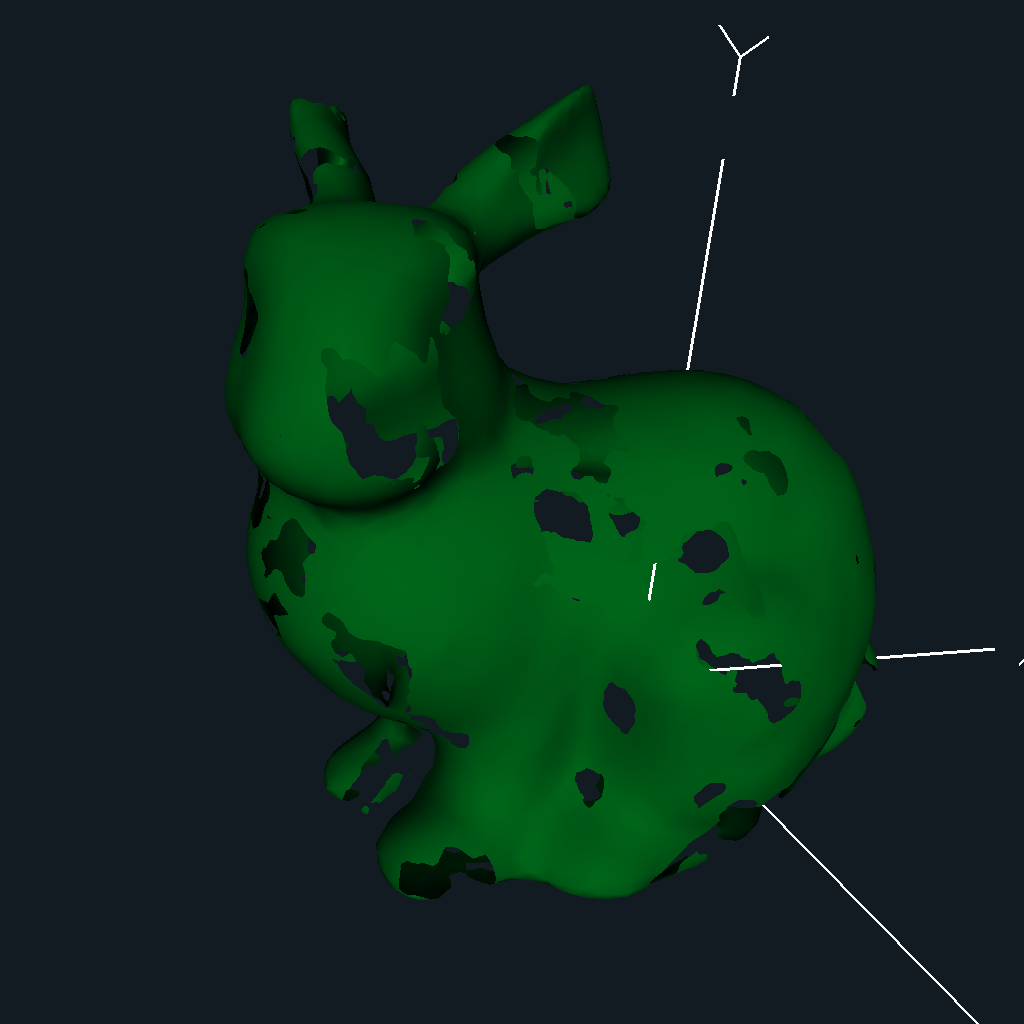
\includegraphics[width=1.0\textwidth]{img/bunny_alpha.png}
    \caption{Bunny with alpha enabled.}
    \label{fig:bunnyalpha}
\end{figure}

\end{document}
